\section{Subject for TOC}
\begin{frame}
    \frametitle{Subject -- Slide 1 Title}
    \begin{block}{Sub-subject 1}
        Text and itemizes here.
    \end{block}
    \begin{block}{Sub-subject 2}
        Text and itemizes here.
    \end{block}
\end{frame}

\begin{frame}[fragile]
    \frametitle{Subject -- Slide 2 Title}
    \begin{columns}[onlytextwidth,t]
        \column{0.49\linewidth}
        \begin{block}{Subject 1}
            Text in the left column.
        \end{block}
        \begin{block}{Subject 2}
            Remember, do not use the following environments for slides! No captions!
            \begin{itemize}
                \item \texttt{figure}
                \item \texttt{table}
            \end{itemize}
        \end{block}
        \begin{block}{Highlighting}
            Use \hl{this} tag to highlight (\verb|\hl{}|).
        \end{block}

        \column{0.49\linewidth}
        \begin{center}
            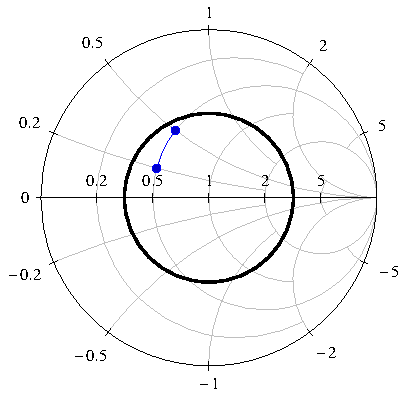
\includegraphics[scale=0.7]{img/smithchart}
        \end{center}
        Here is second column!
    \end{columns}
\end{frame}
